\documentclass[10pt, a4paper]{article}

\usepackage[utf8]{inputenc}
\usepackage[greek, english]{babel}
\usepackage{alphabeta}
\usepackage{libertine}
\usepackage{graphicx}
\usepackage{biblatex}
\usepackage{wrapfig}
\usepackage{hyperref}
\usepackage[table]{xcolor}
\usepackage{mathptmx} % Times New Roman
\usepackage{makecell}
\usepackage{setspace}

\pagenumbering{arabic}
\onehalfspacing % Set line spacing to 1.5

\newcommand{\linkstyle}[1]{\color{blue}\underline{#1}}

\graphicspath{ {./resources/} }

\addbibresource{refs.bib}


\title{\Huge A Comprehensive Study on US College Admissions  }

\author{\large Tsirmpas Dimitris\\Athens University of Economics and Business\\Department of Informatics}


\begin{document}
	
	\begin{titlepage}
		\maketitle
		\begin{center}
					
			
\includegraphics[width=1\textwidth]{aueb_logo.jpg}
			
			\large Athens University of Economics and Business
			
			\large Department of Statistics
			
			\large Greece
		\end{center}
	
	\end{titlepage}
	
	\tableofcontents
	\newpage
	
	\section{Abstract}
	US College Admissions have and continue to be a subject of great debate among scholars and analysts. Such educational institutions have an interest in selecting the most qualified applicants using limited data, while the applicants themselves often protest admission requirements, especially those deemed discriminatory in nature. In this study we discover relationships between the candidate's gender and previous program and their overall test scores. We also identify a positive correlation between test scores, which we attribute to a common, unknown variable called "Competence".
	
	
	\section{Introduction}
	
	The aim of this study is to investigate possible links and relationships between a candidate's characteristics and their performance in multiple standardized tests. We employ a random sample of 200 students who applied to continue their studies in their respective universities. Their application consisted of three standardized tests testing their skills and knowledge in mathematics, social studies and creative writing. An overview of the data contained can be found in Table \ref{tab::dataset}. 
	
	The data and replication code can be found in our GitHub repository \footnote{\url{https://github.com/dimits-exe/college_analysis}}. We make the assumption that the dataset has been acquired through random, unbiased sampling. We also make the assumption that the records using different IDs represent different students (and as such are considered independent samples).
	
	The study is structured as follows: In Section \ref{sec::exploratory} we make general observations about our data, identify key relationships and form our first hypotheses. We follow up these hypotheses in Section \ref{sec::var_cors} with robust analyses and in Section \ref{sec::models} by employing various regression models. Section \ref{sec::conclusions} features an overview and discussion about our findings. Finally, we include graphs, tables and supporting documents in the report's Addendum (Section \ref{sec::addendum}).
	
	
	\section{Exploratory Analysis}
	\label{sec::exploratory}
	
	\begin{table}
		\centering
		\rowcolors{2}{gray!25}{white}
		\begin{tabular}
			{ |p{1cm} p{1cm} p{5cm} p{3cm}| }
			\hline
			\textbf{Name} & \textbf{Type} & \textbf{Description} & \textbf{Range}\\
			\hline
			Id  & Nominal & The student's ID & [1-200] \\
			Gender  & Binary & The student's gender & \{male, female\} \\
			Race  & Nominal & The student's race & \{white, latin-american, asian, african-american\} \\
			Schtype  & Binary & The type of the student's secondary education institution & \{public, private\} \\
			Prog  & Nominal & The student's previous study cycle  & \{general, vocation, academic \} \\
			Write  & Numeric & The grade on the writing test  & [0-100] \\
			Math  & Numeric & The grade on the mathematics test  & [0-100] \\
			Socst  & Numeric & The grade on the social studies test & [0-100] \\
			\hline
		\end{tabular}
		\caption{An overview of the data used in this study.}
		\label{tab::dataset}
	\end{table}
	
	
	The numerical variables contained in the dataset are described in Table \ref{tab::summary_stats}. We observe that they are all almost symmetrical ($-0.5 \leq skew \leq 0.5$), and feature moderate negative (right) skewness with a mean/median hovering just above a score of 50. This indicates most students score around the baseline, most of which pass the exams with a mediocre grade.
	
	\begin{table}
		\centering
		\rowcolors{2}{gray!25}{white}
		\begin{tabular}
			{ |p{1cm} p{0.5cm} p{0.7cm} p{0.5cm} p{1cm} p{0.7cm} p{0.5cm} p{0.5cm} p{0.5cm} p{0.5cm} p{0.5cm}| }
			\hline
			\textbf{Var.} & \textbf{Obs.} & \textbf{Mean} & \textbf{Std} & \textbf{Median} & \textbf{Trim} & \textbf{Min} & \textbf{Max} & \textbf{Skew} & \textbf{Kurt} & \textbf{SE}\\
			\hline
			Write & $200$ & $52.77$ & $9.48$ & $54$ & $53.36$ & $31$ & $67$ & $-0.47$ & $-0.78$ & $0.67$ \\
			Math & $200$ & $52.65$ & $9.37$ & $52$ & $52.33$ & $33$ & $75$ & $0.28$ & $-0.69$ & $0.66$ \\
			Socst & $200$ & $52.41$ & $10.74$ & $52$ &$ 52.99$ & $26$ & $71$ & $-0.38$ & $-0.57$ & $0.76$ \\
			\hline
		\end{tabular}
		\caption{Summary statistics on the numerical data used in the study.}
		\label{tab::summary_stats}
	\end{table}
	
	We next study relationships between the candidates' characteristics (not including test scores). We run $\chi^2$ tests on \textit{Gender, Race, Program} and \textit{School Type}. The only statistically significant relationship in our dataset is between \textit{School Type} and \textit{Program} ($p\_value = 0.015$), which can be seen in Table \ref{tab::chisq}.
	
	\begin{table}
		\centering
		\rowcolors{2}{gray!25}{white}
		\begin{tabular}
			{ |p{2cm} | p{1.2cm} p{1.2cm} p{1.2cm} | p{1.2cm} | }
			\hline
			\multicolumn{5}{|c|}{\textbf{Previous Program}}\\
			\hline
			\textbf{School Type} & \textbf{general} & \textbf{academic} & \textbf{vocation} & \textbf{Total}\\
			\hline
			\textbf{public} & \makecell{39 \\ $23.2\%$} & \makecell{81 \\ $48.2\%$} & \makecell{48 \\ $28.6\%$} & \makecell{168 \\ $100\%$} \\
			\textbf{private} & \makecell{6 \\ $18.8\%$} & \makecell{24 \\ $75\%$} & \makecell{2 \\ $6.2\%$} & \makecell{32 \\ $100\%$}\\
			\hline
			\textbf{Total} & \makecell{45 \\ $22.5\%$} & \makecell{105 \\ $52.5\%$} & \makecell{50 \\ $25\%$} & \makecell{200 \\ $100\%$}\\
			\hline
		\end{tabular}
		\caption{$\chi^2$ test between \textit{School Type} and \textit{Program}. Notice the overwhelming majority of candidates who attended private schools having an academic background prior to applying.}
		\label{tab::chisq}
	\end{table}
	
	
	Finally, we study the relationships between the three subjects. As shown in Table \ref{tab::corr}, there is a very statistically significant ($p\_value = 0.0000$), positive (Pearson's $r > 0.5$) relationship between all three subjects. This could be indicative of either one of the variables influencing the other, or an unknown, interfering variable which positively affects the three test scores. We hypothesize the latter, as the existence of such a variable indicating the student's general competence in tests makes intuitive sense. We will refer to this potential, unknown variable as \textit{"Competence"} in this report.
	
	Since the three subjects are strongly correlated we can explore correlations between the rest of the factors and any of the tests, assuming that a correlation with one strongly indicates with the other two as well. 
	
	We notice a probable correlation between gender and writing scores, as shown in Figure \ref{fig::write_gender}, as well as between the student's program and writing scores, as shown in Figure \ref{fig::write_prog}.
	
	\begin{table}
		\centering
		\rowcolors{2}{gray!25}{white}
		\begin{tabular}
			{ |p{2.5cm} | p{2.5cm} | p{2.5cm}  | p{2.5cm} | }
			\hline
			& \textbf{Writing} & \textbf{Math} & \textbf{Social Studies} \\
			\hline
			\textbf{Writing} & \cellcolor{darkgray} & \cellcolor{darkgray} & \cellcolor{darkgray} \\
			\hline
			\textbf{Math} & \makecell{$0.62$\\ $0.000$ ****} & \cellcolor{darkgray} & \cellcolor{darkgray}\\
			\hline
			\textbf{Social Studies} & \makecell{$0.60$\\ $0.000$ ****} & \makecell{$0.54$\\ $0.000$**** \\} &\cellcolor{darkgray}\\
			\hline
		\end{tabular}
		\caption{Pearson's correlation coefficient (Holm's correction) between the tests and their p\_values. Stars indicate significance scores: $>1$:'', $0.1$:'*', $0.01$: '**', $0.001$: '***', $<0.0001$: '****'.}
		\label{tab::corr}
	\end{table}
	
	\begin{figure}
		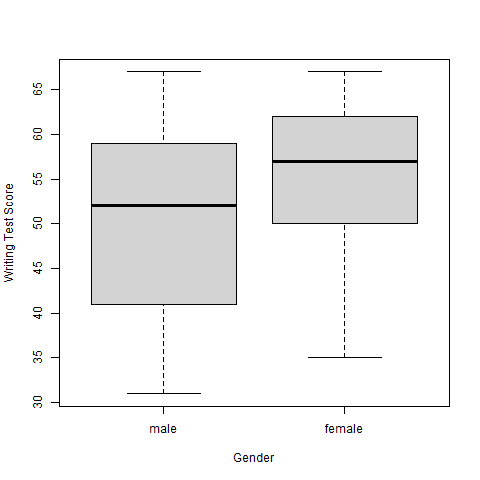
\includegraphics[width=6cm]{write_genre_boxplot.png}
		\centering
		\caption{Boxplot displaying the writing score by gender.}
		\label{fig::write_gender}
	\end{figure}
	
	\begin{figure}
		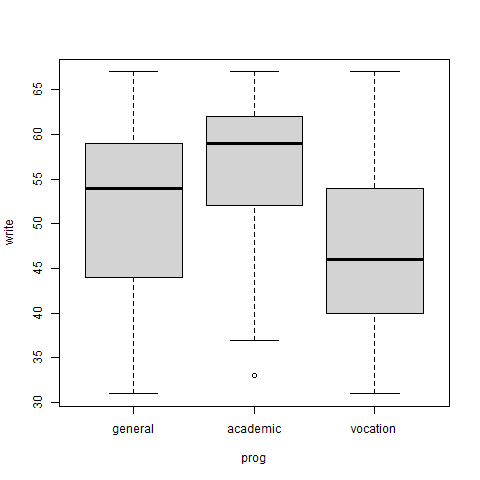
\includegraphics[width=6cm]{write_prog_boxplot.png}
		\centering
		\caption{Boxplot displaying the writing score by current program. Notice the significant differences in means.}
		\label{fig::write_prog}
	\end{figure}
	
	\section{Variable correlations}
	\label{sec::var_cors}
	
	\subsection{Writing scores influenced by gender}
	Our exploratory analysis indicated a possible discrepancy between the results of writing tests between men and women, as well as between different programs. We thus investigate whether gender and the candidate's current program play a role in writing test score.
	
	We begin by verifying the preconditions necessary for the standard t-test in order to compare the genders' scores. We compute the mean differences of the samples by subtracting the global mean by the women's scores \parencite{means}, and conclude they are not normal (Shapiro-Wilk normality test, $p\_value = 0.0024$). The variances are not homogeneous (Levene's test $p\_value = 0.0022$), although this should not dissuade us from using a parametric t-test since the relatively large sample size ($N=200$) and balanced groups ($N_{women} = 109, N_{men} = 91$) means the precondition's violation is not significant \parencite{variances}. We will use a non-parametric test since the distribution of the differences do not have a normal kurtosis (Jarque-Bera Normality Test \cite{jarque}, $p\_value=0.026$), and thus their mean is not suitable.
	
	We conclude there is a statistically significant difference between the writing scores of men and women (Wilcoxon Rank Sum Test, $p\_value = 0.0009$) with women having on average 5 more score than men (Wilcoxon Rank Sum Test with $H_a = less$, $p\_value = 0.0004$).
	
	
	\subsection{Writing scores influenced by previous program}
	We will now verify the preconditions for the parametric ANOVA test in order to test which programs are correlated with the writing tests' scores. The variances of the residuals are homogeneous (Levene's test $p\_value = 0.0022$), but not normal (Shapiro-Wilk normality test, $p\_value = 0.002$). We will thus use a non-parametric test.
	
	We discover there is a statistically significant difference between the groups (Kruskall-Wallis rank sum test, $p\_value=4e-08$). We can consult the boxplots in Figure \ref{fig::write_prog}, where we observe significant differences between all three groups.
	
	
	\section{Predictive / interpretative models}
	\label{sec::models}
	
	
	\subsection{Building the base model}
	Having confirmed our hypotheses regarding the relationships between the various variables and the writing test scores, we attempt to build a model which will estimate a candidate's math and social study scores, testing our hypothesis that the three scores are influenced by the same external factors. 
	
	Since there seem to be strong correlations between most independent variables and the writing scores, and since we already established a strong correlation between the scores themselves (attributed to the candidate's \textit{"Competence"}), we will be using a simple, Ordinary Least Squares (OLS) model.
	
	We initially build an OLS model estimating the writing scores which involves all the available variables. This model exhibits a good fit ($R^2_{adj} = 0.4753, F= 37.06 p\_value=2.2e-16, df=194$). We also verify all the preconditions for the regression model; the residuals appear to be normal (Shapiro-Wilk normality test $p\_value = 0.2099$), homogeneous (Levene's Test, $p\_value = 0.1057$) and non-correlated (Durbin-Watson test, $p\_value=0.236$) and there are no significant outliers (see Addendum).
	
	Our current model exhibits high confidence about the gender ($p\_value_{female} = 0.0056$), previous program  ($p\_value_{progacademic} = 0.0025$), writing scores ($p\_value_{write} = 3.57e-08$), social study scores ($p\_value_{socst} = 0.0053$) and the constant ($p\_value_{intercept} = 8.29e-09$). However, it exhibits low confidence about the candidate's race ($p\_value_{raceasian} = 0.05$) and no confidence about his school type ($p\_value=0.6502$). In order to build an optimal model, we consider dropping these two variables. Dropping the candidate's race along with the school type leads to a slight decrease of $R^2_{adj} = 0.4753$. Dropping only the school type on the other hand leads to an improved $R^2_{adj} = 0.4882$. Since the model maintains its confidence about the other variables, we keep this model as the optimal one. A summary of the optimal model can be found in Table \ref{tab::lm_math_peeking}.
	
	We now follow the same procedure for the social studies test. We fit a model involving all available variables, which explains our sample to a decent degree ($R^2_{adj} = 0.4535, F= 17.7 p\_value=2.2e-16, df=188$). We detect an outlier in our precondition verification, a student with an above-average grade in writing but an abysmal one in social studies. Since this individual exerts a significant influence in our model (as it is largely dependent on the writing scores for its estimations) we remove them from the sample. The other preconditions are met, the residuals are sufficiently normal (Shapiro-Wilk normality test $p\_value = 0.0125$), homogeneous (Levene's Test, $p\_value = 0.3394$) and non-correlated (Durbin-Watson test, $p\_value=0.678$).
	
	As mentioned above, this model is reliant on the math and especially on the writing scores, while the rest of the variables are mostly non-statistically significant. We thus employ a stepwise procedure in order to eliminate variables deemed statistically insignificant while retaining, or increasing our models goodness of fit. A summary of the resulting model can be found in Table \ref{tab::lm_socst_peeking}.
	
	The results seem to verify our main hypothesis, that the test scores are predominately caused by the unknown "Competence" value. While other variables such as the candidate's past program, have a statistically significant influence in our model, we can see that the model's estimations are consistently based on the writing and other-lesson's test scores. We can additionally rule out this relationship being a result of multi-co-linearity between the test variables, as seen in the previous auto-correlations tests.
	
	
% Table created by stargazer v.5.2.3 by Marek Hlavac, Social Policy Institute. E-mail: marek.hlavac at gmail.com
% Date and time: Sat, May 20, 2023 - 3:44:05 PM
\begin{table}[!htbp] \centering 
  \caption{Linear regression model predicting math test scores, taking into 
          account other test scores.} 
  \label{tab::lm_math_peeking} 
\begin{tabular}{@{\extracolsep{5pt}}lc} 
\\[-1.8ex]\hline 
\hline \\[-1.8ex] 
 & \multicolumn{1}{c}{\textit{Dependent variable:}} \\ 
\cline{2-2} 
\\[-1.8ex] & math \\ 
\hline \\[-1.8ex] 
 genrefemale & $-$2.828$^{***}$ \\ 
  & ($-$4.799, $-$0.858) \\ 
  & \\ 
 progacademic & 3.788$^{***}$ \\ 
  & (1.346, 6.229) \\ 
  & \\ 
 progvocation & $-$0.375 \\ 
  & ($-$3.161, 2.410) \\ 
  & \\ 
 write & 0.404$^{***}$ \\ 
  & (0.266, 0.542) \\ 
  & \\ 
 socst & 0.167$^{***}$ \\ 
  & (0.052, 0.283) \\ 
  & \\ 
 raceasian & 4.978$^{*}$ \\ 
  & ($-$0.017, 9.972) \\ 
  & \\ 
 raceafrican-amer & $-$1.103 \\ 
  & ($-$5.104, 2.898) \\ 
  & \\ 
 racewhite & 2.324 \\ 
  & ($-$0.686, 5.334) \\ 
  & \\ 
 Constant & 20.334$^{***}$ \\ 
  & (13.730, 26.938) \\ 
  & \\ 
\hline \\[-1.8ex] 
Observations & 200 \\ 
R$^{2}$ & 0.509 \\ 
Adjusted R$^{2}$ & 0.488 \\ 
Residual Std. Error & 6.702 (df = 191) \\ 
F Statistic & 24.729$^{***}$ (df = 8; 191) \\ 
\hline 
\hline \\[-1.8ex] 
\textit{Note:}  & \multicolumn{1}{r}{$^{*}$p$<$0.1; $^{**}$p$<$0.05; $^{***}$p$<$0.01} \\ 
\end{tabular} 
\end{table} 

	
% Table created by stargazer v.5.2.3 by Marek Hlavac, Social Policy Institute. E-mail: marek.hlavac at gmail.com
% Date and time: Sat, May 27, 2023 - 7:11:52 PM
\begin{table}[!htbp] \centering 
  \caption{Linear regression model predicting social study test scores, taking into 
          account other test scores.} 
  \label{tab::lm_socst_peeking} 
\begin{tabular}{@{\extracolsep{5pt}}lc} 
\\[-1.8ex]\hline 
\hline \\[-1.8ex] 
 & \multicolumn{1}{c}{\textit{Dependent variable:}} \\ 
\cline{2-2} 
\\[-1.8ex] & socst \\ 
\hline \\[-1.8ex] 
 progacademic & 2.276 \\ 
  & p = 0.137 \\ 
  & \\ 
 progvocation & $-$2.669 \\ 
  & p = 0.118 \\ 
  & \\ 
 write & 0.446$^{***}$ \\ 
  & p = 0.00000 \\ 
  & \\ 
 math & 0.242$^{***}$ \\ 
  & p = 0.004 \\ 
  & \\ 
 Constant & 15.610$^{***}$ \\ 
  & p = 0.0003 \\ 
  & \\ 
\hline \\[-1.8ex] 
Observations & 200 \\ 
R$^{2}$ & 0.441 \\ 
Adjusted R$^{2}$ & 0.429 \\ 
Residual Std. Error & 8.111 (df = 195) \\ 
F Statistic & 38.416$^{***}$ (df = 4; 195) \\ 
\hline 
\hline \\[-1.8ex] 
\textit{Note:}  & \multicolumn{1}{r}{$^{*}$p$<$0.1; $^{**}$p$<$0.05; $^{***}$p$<$0.01} \\ 
\end{tabular} 
\end{table} 

	
	
	\subsection{Identifying test score causation}
	
	The results above, although encouraging, do not rule out the alternative hypothesis we posed in the Introduction of this report, that the definite correlation between the test scores is caused by one of the test scores themselves influencing the others. We thus repeat the experiments of the previous subsection while omitting the writing scores. If our alternative hypothesis was correct we would expect our models to no longer have a good performance, while having a much smaller statistical significance on the other lesson's model.
	
	We begin by constructing an OLS regression model which tries to estimate the math score by considering the candidate's characteristics and his scores in the social studies test. Our initial model including all the variables scores a $R^2_{adj} = 0.3999$ score. We next verify all the necessary preconditions; the residuals appear to be normal (Shapiro-Wilk normality test $p\_value = 0.8403$), homogeneous (Levene's Test, $p\_value = 0.1641$) and non-correlated (Durbin-Watson test, $p\_value=0.534$) and there are no significant outliers. 
	
	This model again displays high confidence in the following variables: Race ($p\_value_{raceasian} = 0.002$, $p\_value_{racewhite} = 0.012$), Program ($p\_value_{progacademic} = 0.0005$), Social Study Test Scores ($p\_value_{socst} = 4.25e-09$) and the Constant ($p\_value_{socst} = 2e-16$). By employing a backwards procedure we end up with our final model with a total $R^2_{adj} = 0.4022$, found in Table \ref{tab::lm_math_nopeeking}.
	
	We repeat the procedure for estimating the social study test scores without relying on the writing tests. Our base model, which considers all the available variables, displays a $R^2_{adj} = 0.3393$, which is considerably worse than the respective math model. This may be because of the previously mentioned reliance on the writing scores, which are no longer available to the model. Additionally, similarly to the previous models, the model lacks confidence in almost all other variables; the only statistical significant variable other than the math scores ($p\_value_{math} = 4.25e-09$) and the Constant ($p\_value_{Intercept} = 5.27e-08$) is the candidate's Program ($p\_value_{progvocation} = 0.0283$).
	
	We again verify the preconditions necessary for the linear regression model. The residuals appear to be normal (Shapiro-Wilk normality test $p\_value = 0.7449$), homogeneous (Levene's Test, $p\_value = 0.2314$) and non-correlated (Durbin-Watson test, $p\_value=0.952$) and there are no significant outliers.
	
	Because of the many possible variables that are candidates for removal we can again employ a stepwise model selection algorithm. The best model by AIC keeps only the math and program variables (as expected) but explains less of the data ($R^2_{adj} = 0.3383$). Since the reduction in $R^2_{adj}$ is minimal, and since the new model can reach this score by discarding almost all other variables (which as described above are essentially considered as noise by our model), we will be using this model as optimal (Table \ref{tab::lm_socst_nopeeking}).
	
	These findings seem to contradict our alternative hypothesis. While our models' performance certainly degraded, they still achieve comparable results, with their performance loss being explained by the degree to which \textit{"Competence"} can be measured. In other words, this unknown variable can be approximated more accurately by considering both other tests, instead of just one. This is further proof that our initial hypothesis appears to be correct.
	
	
% Table created by stargazer v.5.2.3 by Marek Hlavac, Social Policy Institute. E-mail: marek.hlavac at gmail.com
% Date and time: Fri, May 19, 2023 - 9:31:05 PM
\begin{table}[!htbp] \centering 
  \caption{Linear regression model predicting social study test scores, 
          without relying on the writing tests} 
  \label{tab::lm_math_nopeeking} 
\begin{tabular}{@{\extracolsep{5pt}}lc} 
\\[-1.8ex]\hline 
\hline \\[-1.8ex] 
 & \multicolumn{1}{c}{\textit{Dependent variable:}} \\ 
\cline{2-2} 
\\[-1.8ex] & math \\ 
\hline \\[-1.8ex] 
 raceasian & 8.074$^{***}$ \\ 
  & p = 0.003 \\ 
  & \\ 
 raceafrican-amer & $-$1.261 \\ 
  & p = 0.567 \\ 
  & \\ 
 racewhite & 4.026$^{**}$ \\ 
  & p = 0.015 \\ 
  & \\ 
 progacademic & 4.726$^{***}$ \\ 
  & p = 0.0005 \\ 
  & \\ 
 progvocation & $-$1.039 \\ 
  & p = 0.499 \\ 
  & \\ 
 socst & 0.335$^{***}$ \\ 
  & p = 0.000 \\ 
  & \\ 
 Constant & 29.617$^{***}$ \\ 
  & p = 0.000 \\ 
  & \\ 
\hline \\[-1.8ex] 
Observations & 200 \\ 
R$^{2}$ & 0.420 \\ 
Adjusted R$^{2}$ & 0.402 \\ 
Residual Std. Error & 7.243 (df = 193) \\ 
F Statistic & 23.318$^{***}$ (df = 6; 193) \\ 
\hline 
\hline \\[-1.8ex] 
\textit{Note:}  & \multicolumn{1}{r}{$^{*}$p$<$0.1; $^{**}$p$<$0.05; $^{***}$p$<$0.01} \\ 
\end{tabular} 
\end{table} 

	
% Table created by stargazer v.5.2.3 by Marek Hlavac, Social Policy Institute. E-mail: marek.hlavac at gmail.com
% Date and time: Sat, May 27, 2023 - 7:11:54 PM
\begin{table}[!htbp] \centering 
  \caption{Linear regression model predicting social study test scores, 
          without relying on the writing tests.} 
  \label{tab::lm_socst_nopeeking} 
\begin{tabular}{@{\extracolsep{5pt}}lc} 
\\[-1.8ex]\hline 
\hline \\[-1.8ex] 
 & \multicolumn{1}{c}{\textit{Dependent variable:}} \\ 
\cline{2-2} 
\\[-1.8ex] & socst \\ 
\hline \\[-1.8ex] 
 progacademic & 2.833$^{*}$ \\ 
  & p = 0.085 \\ 
  & \\ 
 progvocation & $-$3.829$^{**}$ \\ 
  & p = 0.037 \\ 
  & \\ 
 math & 0.486$^{***}$ \\ 
  & p = 0.000 \\ 
  & \\ 
 Constant & 26.285$^{***}$ \\ 
  & p = 0.000 \\ 
  & \\ 
\hline \\[-1.8ex] 
Observations & 200 \\ 
R$^{2}$ & 0.348 \\ 
Adjusted R$^{2}$ & 0.338 \\ 
Residual Std. Error & 8.733 (df = 196) \\ 
F Statistic & 34.908$^{***}$ (df = 3; 196) \\ 
\hline 
\hline \\[-1.8ex] 
\textit{Note:}  & \multicolumn{1}{r}{$^{*}$p$<$0.1; $^{**}$p$<$0.05; $^{***}$p$<$0.01} \\ 
\end{tabular} 
\end{table} 


	
	\section{Conclusions \& Discussion}
	\label{sec::conclusions}
	
	In this report we studied extensively the relationships between different characteristics of US university applicants. We observed that characteristics such as race, gender, schooling and previous programs are uncorrelated, with the exception of a positive relationship between private schooling and academic background. We verified that female candidates score on average higher than males in writing tests, as well as that the candidate's previous program influences their writing test scores. 
	
	Additionally, we observed a definite positive correlation between candidate test scores. We hypothesized this was the product of an unknown variable, called \textit{"Competence"} which similarly influences all test scores and posed an alternative hypothesis stating that one of the test scores was the cause of the correlation. We show evidence of this variable's existence by constructing linear regression models and disprove the alternative hypothesis by constructing such models without access to the common variable \textit{Writing Score}.
	
	This study highlights that other test scores are consistently robust and important variables when attempting to assess future test scores, even if these test scores are on different disciplines (such as social studies and mathematics). Further research is warranted to check whether past test scores can be used to consistently predict candidate performance, as well as from how far in the past, and within which disciplines these scores would be useful.
	
	We note that these findings are only representative for our sample. Our statistical models were used exclusively as explanatory models and should not be used for prediction. We also note that the relationships presented in this report are only representative of our sample, and should not be generalized for the general population. Finally, we warn against extrapolating any relationships from our tests, since they only imply a correlation, not necessarily causation.
	
	
	\section{References}
	\printbibliography[heading=none]
	
	\newpage
	\section{Addendum}
	\label{sec::addendum}
	
	\subsection{Exploratory Analysis}
	In this section we include tables and figures which were used in the exploratory analysis of the data in the Introduction. 
	
	\begin{figure}
		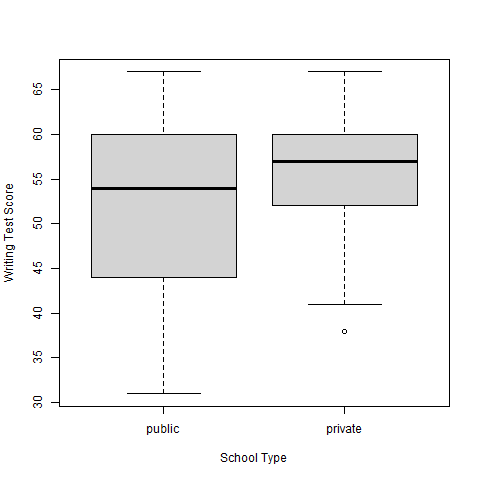
\includegraphics[width=8cm]{write_schtyp_boxplot.png}
		\centering
		\caption{Boxplot displaying the writing score by school type.}
		\label{fig::write_schtyp_boxplot}
	\end{figure}
	
	\begin{figure}
		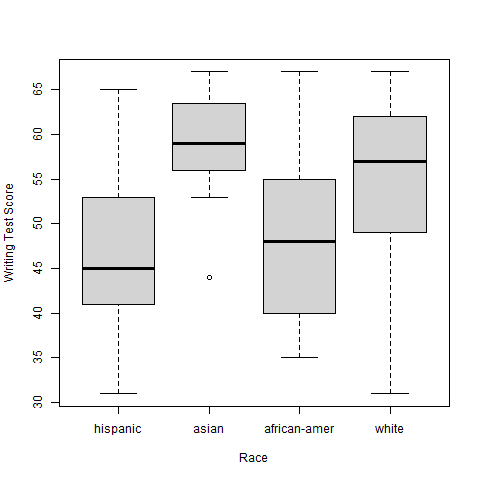
\includegraphics[width=8cm]{write_race_boxplot.png}
		\centering
		\caption{Boxplot displaying the writing score by candidate race.}
		\label{fig::write_race_boxplot}
	\end{figure}
	
	
	\subsection{OLS model preconditions}
	
	In order to visually confirm the normal distribution of the model's residuals, we plot their boxplots for each of the 4 quantiles. We expect these boxplots to resemble those of the normal distribution, centered on $y=0$ and with 95\% of their values not going above/below the $y=1.95$ and $y=-1.95$ respectively. Figures \ref{fig::lm_math_boxplot}, \ref{fig::lm_socst_boxplot} show models including the writing scores. Figures \ref{fig::lm_math_nopeeking_boxplot}, \ref{fig::lm_socst_nopeeking_boxplot} show models including only the other lesson's scores.
	
	\begin{figure}
		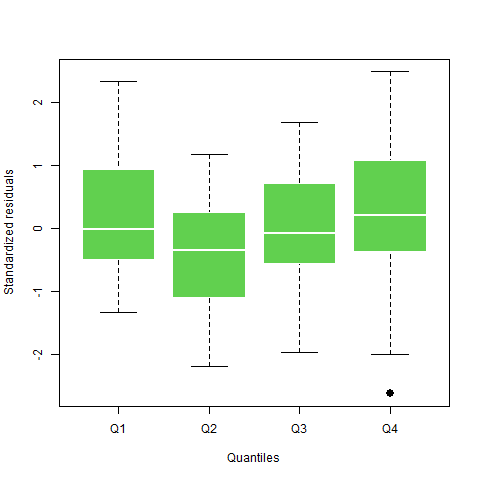
\includegraphics[width=8cm]{lm_math_residual_boxplot.png}
		\centering
		\caption{The normalized residuals of the math model plotted for each of the 4 quantiles.}
		\label{fig::lm_math_boxplot}
	\end{figure}

	\begin{figure}
		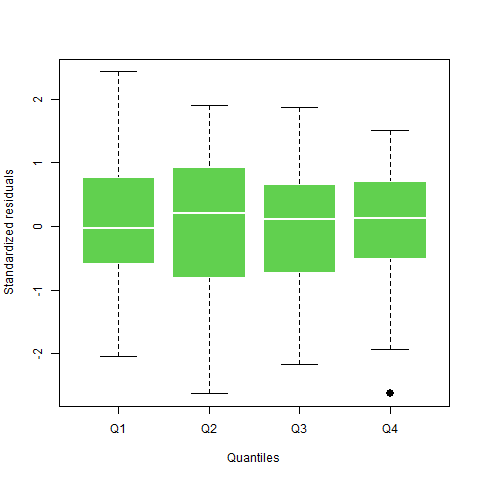
\includegraphics[width=8cm]{lm_socst_residual_boxplot.png}
		\centering
		\caption{The normalized residuals of the social studies model plotted for each of the 4 quantiles. }
		\label{fig::lm_socst_boxplot}
	\end{figure}

	\begin{figure}
		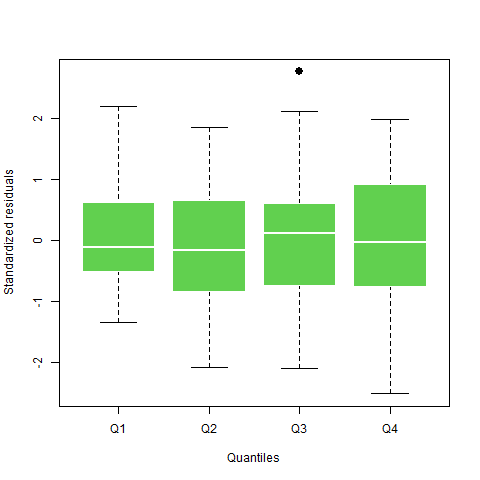
\includegraphics[width=8cm]{lm_math_nopeeking_residual_boxplot.png}
		\centering
		\caption{The normalized residuals of the math model plotted for each of the 4 quantiles. }
		\label{fig::lm_math_nopeeking_boxplot}
	\end{figure}

	\begin{figure}
		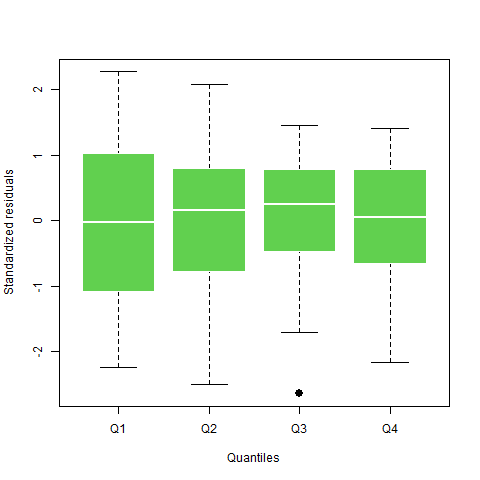
\includegraphics[width=8cm]{lm_socst_nopeeking_residual_boxplot.png}
		\centering
		\caption{The normalized residuals of the math model plotted for each of the 4 quantiles. }
		\label{fig::lm_socst_nopeeking_boxplot}
	\end{figure}


	We also check for outliers by plotting the normalized residuals against the model's estimations. The red lines denote the $y=1.95$ and $y=-1.95$ values respectively and we expect 95\% of the points to be within them. Any value outside of $[-3,3]$ indicates a strong outlier which must be investigated. Figures \ref{fig::lm_math_plot}, \ref{fig::lm_socst_plot} show models including the writing scores. Figures \ref{fig::lm_math_nopeeking_plot}, \ref{fig::lm_sosct_nopeeking_plot} show models including only the other lesson's scores.
	
	 \begin{figure}
	 	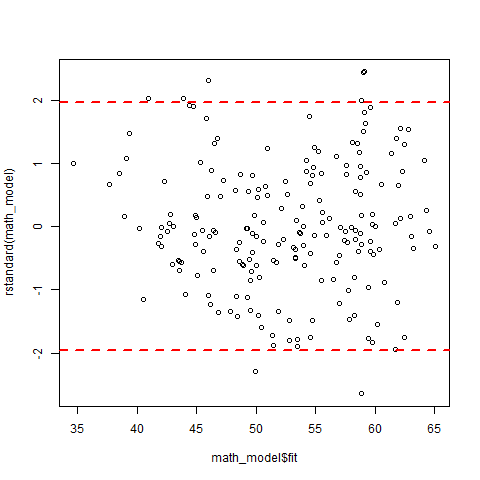
\includegraphics[width=4cm]{lm_math_residual_plot.png}
	 	\centering
	 	\caption{The normalized residuals of the math model plotted against the model's estimations.}
	 	\label{fig::lm_math_plot}
	 \end{figure}
 
	 \begin{figure}
	 	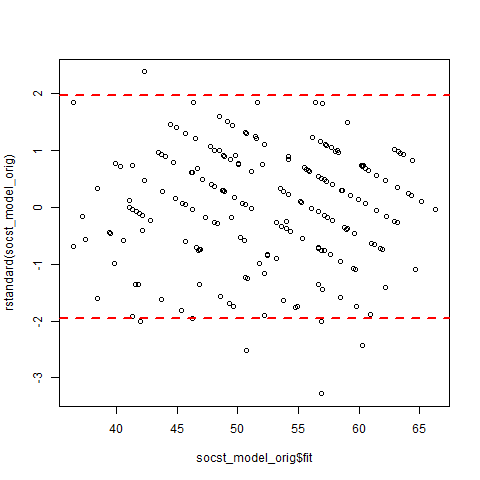
\includegraphics[width=4cm]{lm_socst_residual_plot.png}
	 	\centering
	 	\caption{The normalized residuals of the social studies model plotted against the model's estimations. Notice the one outlier above the $y=3$ line, which represents the data point that was investigated and removed.}
	 	\label{fig::lm_socst_plot}
	 \end{figure}
 
	 \begin{figure}
	 	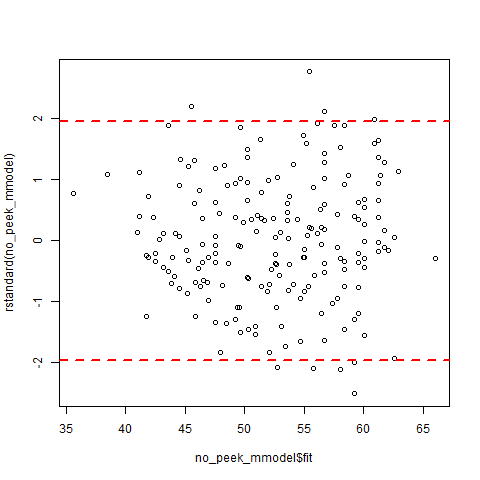
\includegraphics[width=4cm]{lm_math_nopeeking_residual_plot.png}
	 	\centering
	 	\caption{The normalized residuals of the math model plotted against the model's estimations. We notice three potential outliers. These values are considered non-anomalous, as they stray sufficiently away from the $y=3$ and $y=-3$ brackets, and are to be expected in a sample of 200 values.}
	 	\label{fig::lm_math_nopeeking_plot}
	 \end{figure}
 
	 \begin{figure}
	 	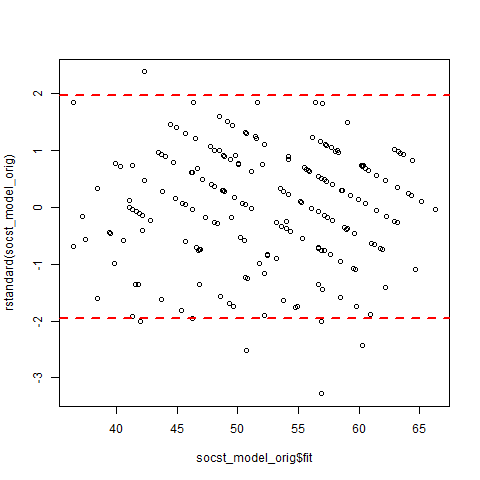
\includegraphics[width=4cm]{lm_socst_residual_plot.png}
	 	\centering
	 	\caption{The normalized residuals of the social studies model (without the writing scores variable) plotted against the model's estimations. We don't consider the values above and below the $y=3$ and $y=-3$ brackets respectively for the same reasons as in Figure \ref{fig::lm_math_nopeeking_plot}.}
	 	\label{fig::lm_sosct_nopeeking_plot}
	 \end{figure}
	
\end{document}